%%    VLNKA <fileinput>  KkSsVvZzOoUuAaIi
\documentclass[12pt, a4paper, oneside]{article}
\usepackage{czech}
\usepackage[center]{caption}
\usepackage[utf8]{inputenc}
\usepackage{wrapfig} % nastavení obtékání textu
\usepackage{graphicx} % nastavení grafiky, matematiky
\usepackage{float}
\usepackage{amsmath}
\usepackage{amssymb}
\usepackage{bbding}
\usepackage{enumitem}
\usepackage{fancyvrb}
\usepackage{marginnote}
\usepackage{marginfix}
\usepackage{breakurl}
\usepackage{listings}
\usepackage{color}
\usepackage{tocloft} % přidá tečky do obsahu ke kapitolám /sekcím
\usepackage{pst-barcode}
\usepackage[latex=-shell-escape]{auto-pst-pdf} % uncomment this if used with pdflatex
\usepackage[bookmarksopen,colorlinks,plainpages=false,linkcolor=black,urlcolor=blue,citecolor=black,filecolor=black,menucolor=black,unicode=true,breaklinks]{hyperref}
\usepackage[backend=biber,bibstyle=numeric,sorting=none,date=long,dateabbrev=false,texencoding=utf8,bibencoding=utf8]{biblatex}

%%%% Bibliography
\addbibresource{../text.bib}
\DeclareFieldFormat[online]{url}{Dostupné na World Wide Web:\\* \href{#1}{\textless\nolinkurl{#1}\textgreater}}
\DeclareFieldFormat[online]{title}{\It{#1} [online]}
\DeclareNameAlias{default}{last-first}

\renewbibmacro*{url+urldate}{%
   \printurldate%
   \printfield{url}
}

\newcommand*{\mkbibrangeMYSTYLE}[1]{%
  \printtext{%
    \mkbibdateMYSTYLE{#1year}{#1month}{#1day}%
    \iffieldundef{endyear}% is it a range?
    {}%
    {\iffieldequalstr{#2endyear}{}% open-ended range?
      {\mbox{\bibdatedash}}%
      {\bibdatedash%
        \mkbibdateMYSTYLE{#1endyear}{#1endmonth}{#1endday}%
      }%
    }%
  }%
}
\newcommand*{\mkbibdateMYSTYLE}[3]{%
  [cit. \mbox{%
  \thefield{#1}%
  \iffieldundef{#2}{}{-\thefield{#2}}%
  \iffieldundef{#3}{}{-\thefield{#3}}}]. %
}
\ExecuteBibliographyOptions{urldate=MYSTYLE}

%%%% Minted
\definecolor{lightgray}{RGB}{240,240,240}
\definecolor{darkgray}{rgb}{.4,.4,.4}
\definecolor{purple}{rgb}{0.65, 0.12, 0.82}
\definecolor{darkgreen}{RGB}{0,150,0}

\renewcommand{\listingscaption}{Příklad}
\renewcommand{\listoflistingscaption}{Příklady}

%%%% Dimensions
\addtolength{\textwidth}{-2mm}
\addtolength{\hoffset}{4mm}  % posun textu kvůli kroužkové vazbě  

\setlength{\intextsep}{5mm} % nastavení mezery okolo obrázků
\marginparsep=15pt
\linespread{1.3}
\unitlength=1mm % nastavení volby jednotek 

% nastavení příkazu >\figcaption pro popis čehokoli, jako by to byly obrázky 
\makeatletter
\newcommand\figcaption{\def\@captype{figure}\caption}
\makeatother

% definice příkazů
\newcommand{\D}{\medskip \noindent} % nový odstavec v "americkém" formátování 
\newcommand{\B}{\textbf} %tučné písmo
\newcommand{\A}{\mathbf} %tučné písmo v matematickém režimu
\newcommand{\TO}{\ensuremath{\boldsymbol\Omega}} % tučný znak velké omega -- pro ohmy
\newcommand{\I}{\index}  % vytváří položku indexu (asi nepoužijete)
\newcommand{\Deg}[1][]{\ensuremath{{#1}^\circ}} % vysází značku stupně Celsia
\newcommand{\Def}{\footnotesize Definice: \normalsize}
\newcommand{\Pos}{\footnotesize Experiment: \normalsize}
\newcommand{\Odv}{\footnotesize Odvození: \normalsize}
\newcommand{\Vym}{\footnotesize Vymezení pojmu: \normalsize}
\newcommand{\Ob}{obrázek }
\newcommand{\It}{\textit}  % kurzíva
\newcommand{\M}{\mathrm}   % v prostředí rovnic nastaví normální písmo (místo kurzívy ) 
\newcommand{\F}{\footnotesize} % zmenšená velikost písma
\newcommand{\N}{\normalsize} % normální velikost písma
%\newcommand{\U}{\underline}  % podtržené písmo
\newcommand{\e}{\ensuremath} 
\newcommand{\Has}{\textcolor{green}{\CheckmarkBold}}
\newcommand{\NoHas}{\textcolor{red}{\XSolidBrush}}
\newcommand*{\fullref}[1]{\hyperref[{#1}]{\ref*{#1}: \uv{\nameref*{#1}} na straně \pageref{#1}}}
\newcommand*{\attref}[1]{\hyperref[{#1}]{\uv{\nameref*{#1}} na straně \pageref{#1}}}
\newcommand{\qrcode}[1]{%
  \begin{pspicture}(30mm,30mm)%
    \psbarcode{#1}{eclevel=L width=0.85 height=0.85}{qrcode}%
  \end{pspicture}%
}
%\newcommand{\qrcode}[1]{ }
\newcommand{\qrurl}[1]{\url{#1}\marginpar{\qrcode{#1}\vspace{7pt}}}

%%%% Misc
\renewcommand{\cftsecdotsep}{\cftdotsep}

%\hypersetup{pdfencoding=auto}
\urlstyle{rm}
\DefineShortVerb{\|}

%\hyphenation{\-Pusť-me pla-tí hod-no-ty do-sa-dí-me za-da-né dal-ším u-mož-ňu-je}
% dělení slov, kdyby implicitní nevyhovovalo

% konec hlavičky
%%%%%%%%%%%%%%%%%%%%%%%%%%%%%%%%%%%%%%%%%%%%%%%%%%%%%%%%%%%%%%%%%%%
%%%%%%%%%%%%%%%%%%%%%%%%%%%%%%%%%%%%%%%%%%%%%%%%%%%%%%%%%%%%%%%%%%%

\begin{document}
~
\vspace{-20mm}
\begin{center}

\Large
\B{MultiROM \\ Nástroj pro instalaci více operačních systémů na jedno mobilní zařízení}
\large

Vojtěch Boček

\end{center}
\section*{Úvod}
\addcontentsline{toc}{section}{Úvod} % přidá položku úvod do obsahu
\label{uvod}
Můj projekt MultiROM je modifikace pro tablety a~telefony původně s~OS Google Android, která umožňuje instalaci více operačních systémů zároveň. MultiROM tedy přidává funkci, která je na stolních počítačích samozřejmostí, ale v~kategorii těchto přenosných počítačů v~naprosté většině případů chybí. Mezi hlavní vlastnosti MultiROM patří zejména:

\begin{itemize}
    \item Možnost instalace libovolného množství operačních systémů na jedno zařízení.
    \item Podpora mnoha operačních systémů, kromě Androidu podporuje například systém Ubuntu Touch nebo Plasma Active.
    \item V~porovnání s~existujícími modifikacemi s~podobným účelem se MultiROM velmi snadno používá a~často má mnohem větší možnosti.
    \item Dokáže vedlejší systémy instalovat jak do vnitřní paměti, tak na USB disk připojený k~zařízení.
\end{itemize}

\section{Motivace}
Abych mohl vysvětlit důvod, proč je multi-boot na mobilních zařízeních užitečný, musím nejdříve upozornit na možnosti, které tato zařízení mají.

Tablety a~telefony s~platformou Google Android lze na rozdíl od jiných mobilních systémů relativně snadno upravovat. Uživatelé na nich mohou získat přístup k~tzv. superuživateli\footnote{Uživatel, který má práva přistupovat a~měnit všechny části systému, je možné ho připodobnit k~uživateli \It{Administrátor} v~MS Windows. V~Linuxu se jmenuje \It{root}.} a~dále pak upravovat software na zařízení jakýmkoliv způsobem chtějí. Toto společně s~faktem, že velká část OS Android má otevřené zdrojové kódy, vedlo ke vzniku obrovské komunity programátorů a~nadšenců, kteří tyto zařízení různými způsoby upravují a~vylepšují. Jedním z~\uv{produktů} této komunity jsou celé upravené distribuce Androidu pro které se ustálilo označení \uv{ROM}.

\subsection{Android ROM}
ROM lze přirovnat k~distribucím Linuxu, jak je známe ze stolních počítačů. Jejich základem jsou obvykle zdrojové kódy z~AOSP\cite{aosp}\footnote{\It{Android Open Source Project} -- označení pro otevřenou část zdrojových kódů OS Android}, které si autoři upravují podle svých představ -- přidávají optimalizace pro zrychlení celého systému, přidávají další možnosti personalizace pro uživatele, mění prvky uživatelského rozhraní a~mnoho dalšího. Na zařízeních, která již nejsou podporované výrobcem, mohou být ROM jediným způsobem, jak na ně přinést novější verze OS Android.

\subsection{Další operační systémy}
Kromě Androidu existují i~další mobilní operační systémy, například Ubuntu Touch\cite{utouch}, Mozilla Firefox OS\cite{firefoxos} a~další. Tyto systémy často používají zařízení původně prodávaná s~Androidem jako testovací, zejména kvůli jejich snadné dostupnosti a~relativně nízké ceně. Pro tablet Google Nexus 7 dokonce existuje plná verze Linuxové distribuce Ubuntu, díky které je možné tento tablet po připojení klávesnice a~myši používat jako netbook, s~většinou programů které známe z~PC verze.

\begin{figure}[H]
\begin{center}
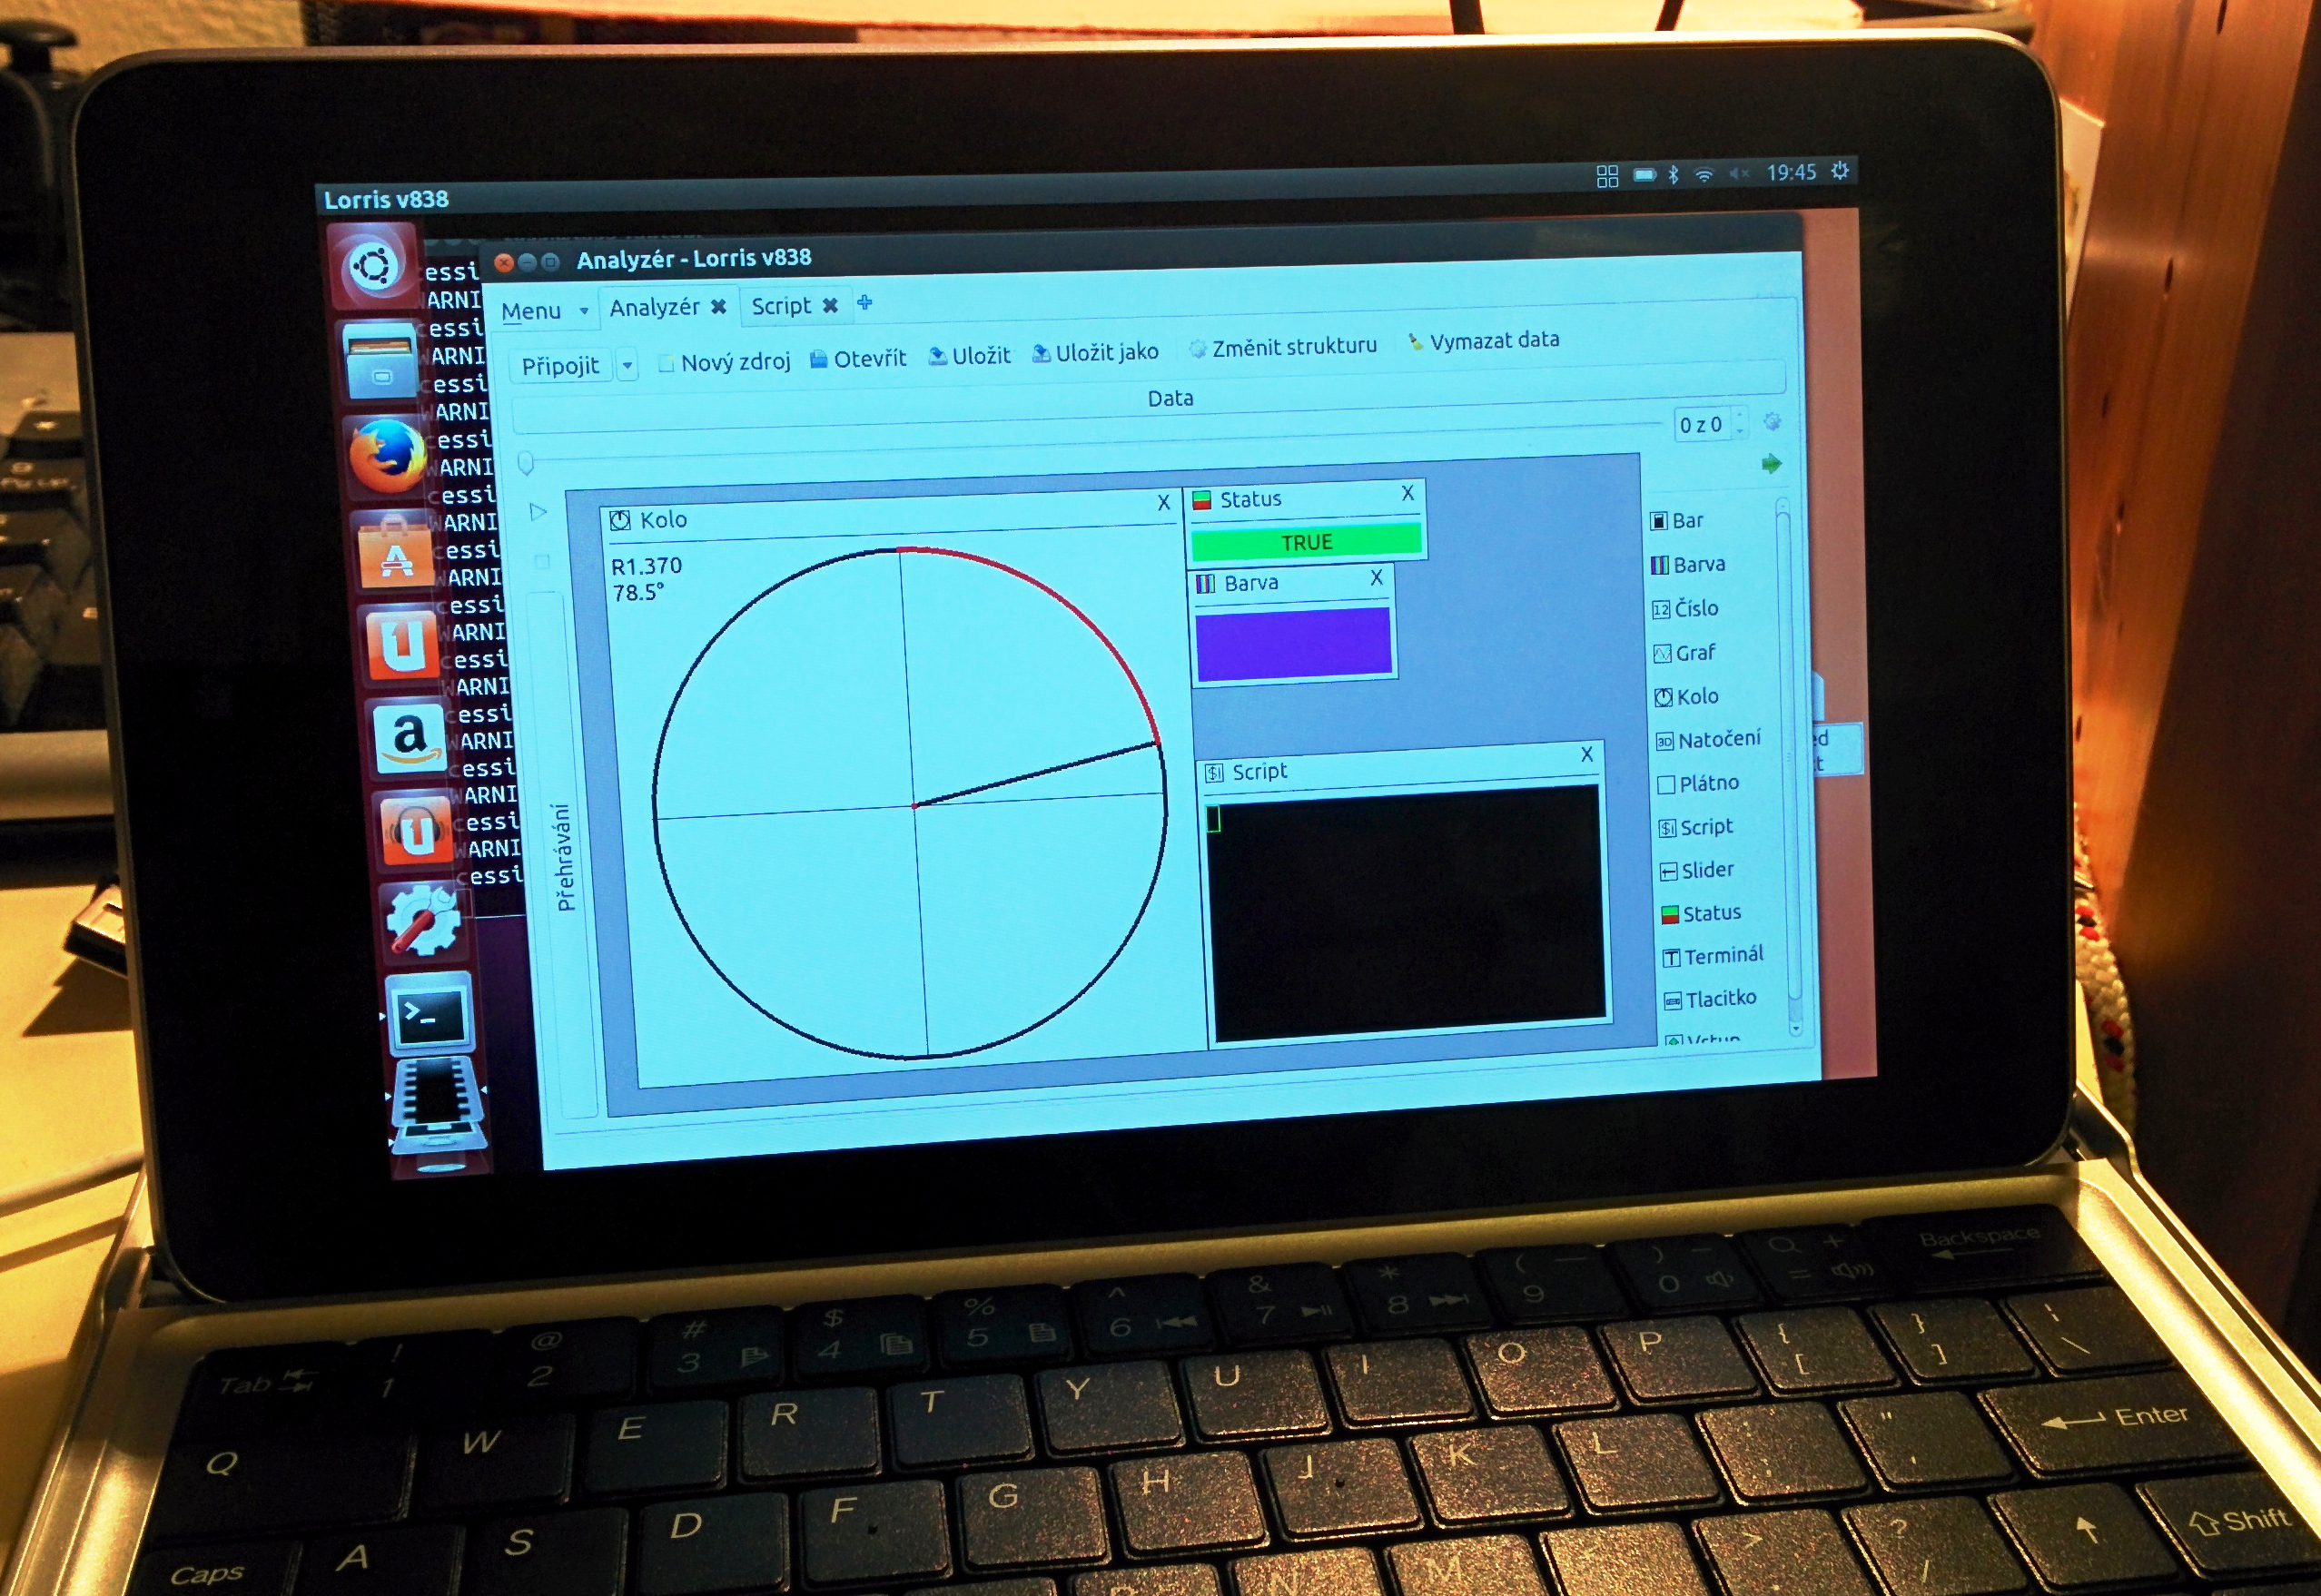
\includegraphics[width=\textwidth]{../img/n7_ubuntu.jpg}
\caption{Ubuntu na tabletu Nexus 7 s~připojenou klávesnicí}
\end{center}
\end{figure}

\subsection{Více systémů na jednom zařízení}
Tyto telefony a~tablety tedy ve většině případů nejsou uzamknuté na jediném, výrobcem vybraném systému a~jeho verzi a~dokáží podobně jako stolní počítače provozovat více typů a~verzí operačních systémů. Chybí jim však možnost mít více systémů nainstalovaných zároveň (dále jen \It{multiboot}). Tato skutečnost pravděpodobně nevadí běžnému uživateli, nicméně pro zkušené uživatele a~vývojáře je \It{multiboot} neocenitelnou funkcí, a~to i~na těchto přenosných zařízeních.

Mohou ho využít například při \B{zkoušení jiných ROM}, kdy ROM vytvořené komunitou mají v~některých případech nové a~velmi zajímavé funkce, nicméně je často vhodné vyzkoušet si danou ROM před tím, než uživatel projde zdlouhavým procesem obnovování všech svých dat do této nové ROM. Toto platí i~pro jiné operační systémy -- příkladem budiž Ubuntu Touch od firmy Canonical, nový operační systém s~ovládáním značně odlišným od Androidu. Řada uživatelů by si tento OS ráda zkusila, nicméně Ubuntu Touch je stále ve vývoji a~není ještě zcela schopný plně nahradit Android. Bez \It{multibootu} by museli museli smazat svůj hlavní OS, což řadu uživatelů odradí.

\section{MultiROM}
Můj projekt MultiROM je modifikací pro zařízení původně s~OS Android, která umožňuje používat více operačních systémů zároveň na jednom zařízení. Skládá se ze čtyř částí, které budou dále důkladně popsány v~samostatných kapitolách:

\begin{enumerate}
    \item \B{boot manager} -- hlavní část tohoto projektu. Zobrazuje se v~průběhu startu zařízení, nechá uživatele vybrat, který operační systém chce spustit a~provede akce nutné ke spuštění tohoto systému.
    \item \B{upravená recovery} -- tato část se stará o~snadnou instalaci a~správu nainstalovaných systémů.
    \item \B{kexec-hardboot patch} -- modifikace Linuxového jádra, která umožňuje nastartovat jiné jádro z~již běžícího, tedy ukončit aktuální operační systém a~spustit nový. Jedná se o nejsložitější část MultiROM, která je klíčová k její funkci, ale v prostoru této synapse bohužel patch nemohu plně popsat.
    \item \B{aplikace pro Android} -- umí rychle a~jednoduše nainstalovat všechny potřebné části MultiROM a~aktualizovat je a~do omezené míry spravovat nainstalované systémy a~také do nich přepnout přímo z~Androidu, bez nutnosti restartovat zařízení a~až poté vybrat systém v~boot manageru.
\end{enumerate}

\newpage
MultiROM je svobodný software, distribuovaný pod licencí GNU GPLv3 (boot manager, recovery a~Android aplikace) a~GNU GPLv2 (kexec-hardboot patch). Zdrojové kódy jsou k~dispozici v~repozitářích na serveru GitHub:
\begin{itemize}
    \item \B{Boot manager:} \\ \qrurl{http://github.com/Tasssadar/multirom}
    \item \B{Recovery:}\\ \qrurl{http://github.com/Tasssadar/Team-Win-Recovery-Project}
    \item \B{Android aplikace}:\\ \qrurl{http://github.com/Tasssadar/MultiROMMgr}
\end{itemize}

Na serveru Github je také k~dispozici wiki s~informacemi jak pro uživatele, tak pro vývojáře kteří chtějí vědět více o~tom jak MultiROM funguje nebo ji chtějí upravit pro svoje zařízení. Je napsaná z~části mnou (zejména články týkající se technických záležitostí) a~z~části členy komunity (hlavně informace o~používání MultiROM).

\begin{itemize}
\item \qrurl{https://github.com/Tasssadar/multirom/wiki}
\end{itemize}

\section{Srovnání s~jinými multiboot nástroji}
Žádný jiný multiboot nástroj pro zařízení řady Nexus, které MultiROM podporuje, neexistuje, proto budu můj projekt srovnávat s~metodami, které jsou běžné pro jiné telefony a~tablety.

Nejčastějším způsobem je tzv. \B{dual-boot kernel}, který spočívá v~upravení \It{init} skriptů a~používání některé z~volných oddílů na zařízení pro umístění druhé ROM (například |/cache|). Do druhého systému se uživatel nabootuje, pokud bude držet některou z~kláves na zařízení, např. snížení hlasitosti. Nevýhody této metody jsou možnost instalace pouze dvou systémů, které navíc musí být jen Android ROM. Dále používá pro obě ROM stejné jádro, které tím pádem musí být s~oběma kompatibilní. To může být často problém, na většině zařízení existují 2 a~více základních druhů ROM, které mezi sebou nejsou kompatibilní.

Méně častá jsou \B{řešení založená na volání kexec}, podobně jako MultiROM. Pro ukládání vedlejších ROM používají obrazy oddílů nebo složky a~často mají i~nějakou formu boot manageru. Jako příklad použiji modifikaci \It{Xperia Boot Menu}\cite{xperia-boot-menu}, která používá kexec-hardboot patch, nicméně nemá upravenou recovery, která by pomáhala s~instalací vedlejších ROM. Tato činnost se tím pádem stává poměrně náročnou.

Dalším populární modifikací je MoDaCo.SWITCH\cite{modaco-switch}, jejíž hlavní předností je sdílení všech dat a~aplikací mezi hlavním a~vedlejším systémem. Jedná se však pouze o~dual-boot, a~to jen mezi dvěma předem určenými ROM -- uživatel si je nemůže vybrat, protože jsou součástí této modifikace. Právě to umožňuje relativně bezproblémové sdílení všech dat mezi oběma systémy, které MultiROM ještě nepodporuje.

Mezi hlavní výhody MultiROM patří zejména \B{velmi snadná instalace a~používání} v~porovnání s~ostatními podobnými modifikacemi. Aplikace pro Android nainstaluje vše potřebné a~udržuje MultiROM aktualizovanou a~další systémy se instalují v~upravené recovery velmi podobně jako bez multibootu -- stačí pouze vybrat ZIP soubor a~stisknout tlačítko. MultiROM dále podporuje téměř \B{jakýkoliv typ operačního systému} -- například pro Nexus 7 existují kromě Androidu balíčky se systémy Ubuntu Touch, Ubuntu Desktop, Plasma Active, WebOS, Tizen, BohdiLinux či ArchLinux. Další důležitou vlastností je možnost \B{instalace jakéhokoliv množství vedlejších systémů}, jediným limitem je velikost paměti. Navíc je možné \B{instalovat i~na USB flash disk}, pokud je interní paměť zařízení vyčerpána.

\newpage
\section{Přijetí MultiROM}
\subsection{XDA Developers fóra}
Server \qrurl{http://xda-developers.com} je největším webem zabývajícím se upravováním Android (ale i~jiných) zařízení. Jeho hlavní částí je fórum, kde vývojáři a~nadšenci vydávají své produkty. Právě zde lze nalézt nejvíce různých druhů ROM a~dalších modifikací.

Hlavním způsobem, jak získává MultiROM nové uživatele a~já komunikuji s~existujícími jsou právě vlákna na XDA fóru. Obsahují popis MultiROM, návod na instalaci, návod k~používání, seznam změn a~odkazy ke stažení. Každé zařízení má své vlastní vlákno:

\begin{itemize}
\item Nexus 7 (2012):\\ \qrurl{http://forum.xda-developers.com/showthread.php?t=2011403}
\item Nexus 7 (2013):\\ \qrurl{http://forum.xda-developers.com/showthread.php?t=2457063}
\item Nexus 4:\\ \qrurl{http://forum.xda-developers.com/showthread.php?p=46223377}
\item Nexus 5:\\ \qrurl{http://forum.xda-developers.com/showthread.php?t=2571011}
\end{itemize}

\subsection{Indiegogo kampaň}
Po vydání nové verze tabletu Nexus 7 v~roce 2013 jsem zaznamenal poměrně velké množství požadavků aby MultiROM podporovala i~toto zařízení. Poskytnout takovou úroveň podpory, kterou bych chtěl (zejména řešení problémů pokud něco nefunguje) je však takřka nemožné, pokud zařízení nevlastním a~nemohu na něm vše testovat. Založil jsem tedy na serveru indiegogo.com\cite{indiegogo} crowdfundingovou kampaň na zakoupení Nexusu 7 a~přidaní kompatibility pro toto zařízení\cite{indiegogo-multirom}. Cílem byla částka \$500 (menší indiegogo nepodporuje). \B{Kampaň byla úspěšná}, celkově se vybralo 562 dolarů a~\B{já jsem svůj \uv{závazek} splnil, a~to i~v~odhadovaném čase} -- verze pro Nexus 7 byla vydána necelý měsíc po skončení kampaně.

% FIXME: zmenšit?
\begin{figure}[H]
\begin{center}
 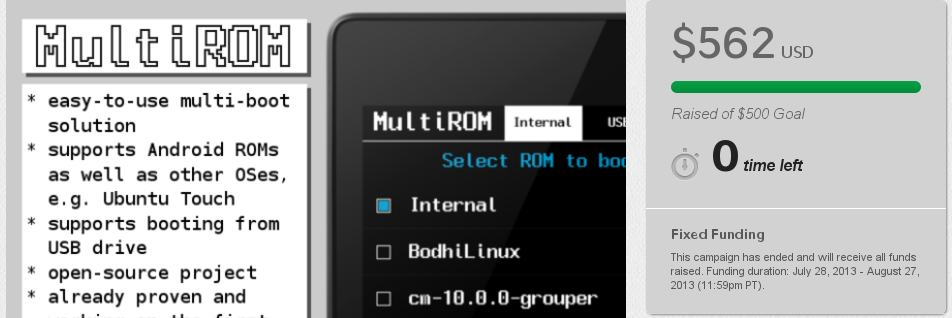
\includegraphics[width=\textwidth]{../img/indiegogo.png}
\caption{Výsledek kampaňe na Indiegogo.com}
\end{center}
\end{figure}

\vspace{-13.5mm}
\subsection{Počet uživatelů}
Ke každé aplikaci v~Obchodě Google Play jsou dostupné i~poměrně podrobné statistiky aktivních uživatelů, a~tak od vydání aplikace pro Android mohu sledovat i~počet uživatelů MultiROM. Tyto statistiky nejsou úplně přesné, protože nezahrnují uživatele, kteří nemají aplikaci nainstalovanou (aplikace není nutnou součástí MultiROM, pouze usnadňuje její používání) ani uživatele některého z~mnou nepodporovaných zařízení.

Na grafu č. \ref{graf-uzivatele} můžete vidět graf \B{aktivních} instalací (nezahrnuje tedy zařízení, ze kterých byla aplikace odinstalována) ke dni 3.\,6.\,2014. Poslední hodnota je \B{19 946 instalací}.

\begin{figure}[H]
\begin{center}
 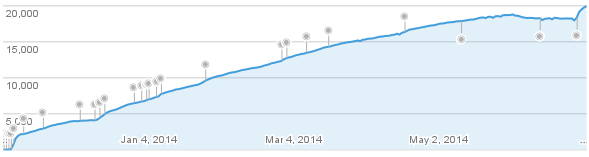
\includegraphics[width=\textwidth]{../img/graph_active_hlavicky.png}
\caption{Graf znázorňující nárůst aktivních instalací}
\label{graf-uzivatele}
\end{center}
\end{figure}

\newpage
\section*{Závěr}
\addcontentsline{toc}{section}{Závěr}
Můj projekt MultiROM se stal až překvapivě úspěšným. Tuto skutečnost přisuzuji zejména, v~porovnání s~ostatními podobnými úpravami, snadnému používání a~takřka žádným nevýhodám oproti stavu, kdy modifikace není nainstalována. Instalaci zvládne díky nabízené aplikaci pro Android i~lehce pokročilý uživatel. Na serveru Youtube má pak k~dispozici několik desítek video návodů, a~to nejen v~angličtině.

Vyzkoušení některého z~méně známých operačních systémů dostupných pro tato přenosná zařízení dříve znamenalo spoustu času stráveného vytvářením záloh a~jejich obnovováním. Díky mému projektu se tento proces značně usnadňuje, a~nepřímo tak pomáhá i~vývojářům těchto systémů, protože více uživatelů si jejich produkt vyzkouší anebo si ho dokonce oblíbí.

Vedlejším produktem mojí práce na MultiROM jsou opravy a~vylepšení projektů, které moje modifikace rozšiřuje nebo se jich jinak dotýká. Většina změn, které nejsou částí MultiROM, byla odeslána do hlavních stromů příslušných projektů a~řada z~nich si našla cestu i~k~uživatelům, kteří MultiROM nemají nainstalovanou. Toto platí zejména o~upravené recovery TeamWin Recovery Project.

MultiROM má po dvou letech od vydaní první verze pro Nexus 7 (2012) téměř 20 tisíc aktivních instalací a~mnoho pozitivních ohlasů od uživatelů. Má za sebou úspěšnou crowdfunding kampaň, na kterou přispívali sami uživatelé a~vývojáři a~díky které se rodina oficiálně podporovaných zařízení z~původního Nexusu 7 rozrostla na celkově 2 tablety a~2 telefony z~řady Google Nexus a~více než dvojnásobek jiných zařízení, která podporují další členové komunity.

V~budoucnu bych chtěl přidat podporu pro další zařízení a~implementovat možnost sdílení aplikací a~jejich dat mezi několika instalacemi operačního systému Android.


\newpage
\voffset=-80pt
\addtolength{\textheight}{70pt}
\addtolength{\footskip}{70pt}
 \section*{PŘÍLOHA A:}
 \section*{Velké obrázky}
 \addcontentsline{toc}{section}{PŘÍLOHA A: Velké obrázky}
 \label{obrazky}

\addtolength{\textheight}{-70pt}
\begin{figure}[H]
\begin{center}
 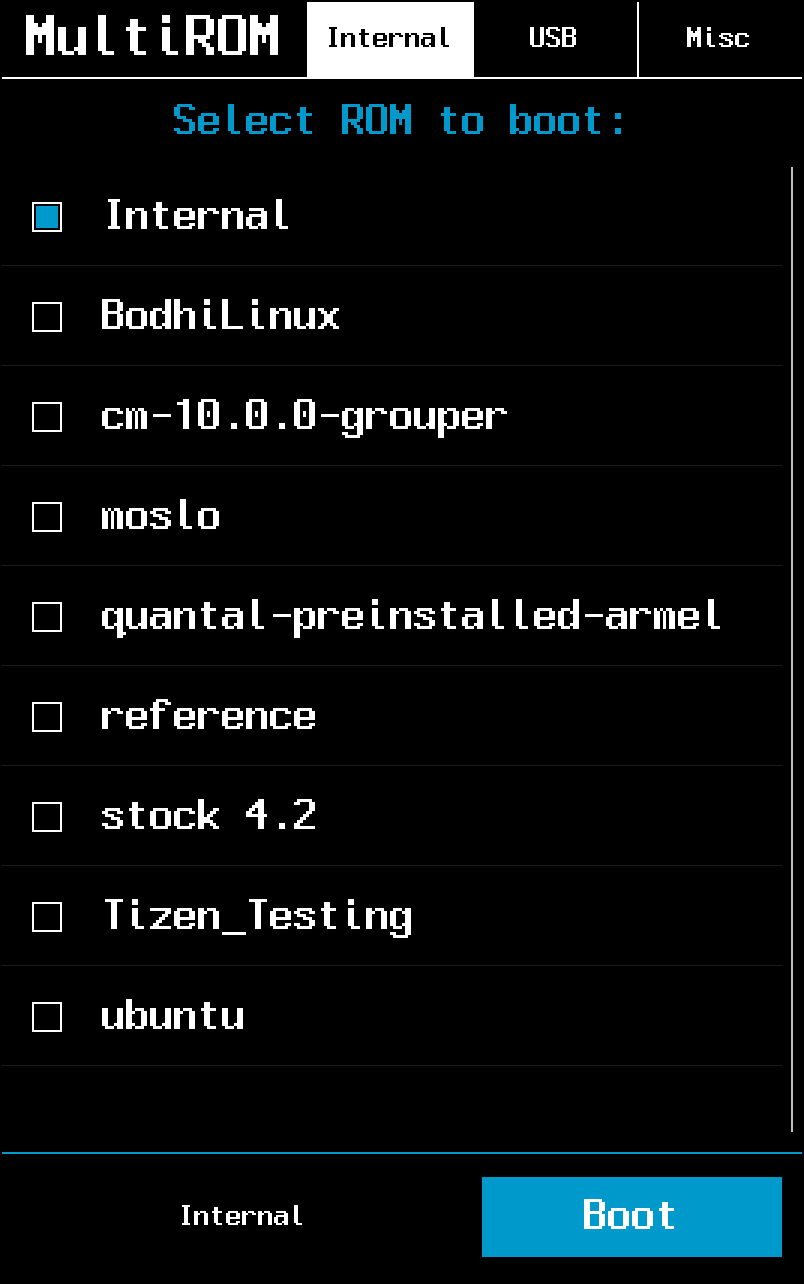
\includegraphics[height=550pt]{../img/boot_manager.png}
\caption{Boot manager: hlavní obrazovka se seznamem systémů}
\end{center}
\end{figure}

\newpage
\voffset=0pt
\addtolength{\footskip}{-70pt}

\begin{figure}[H]
\begin{center}
 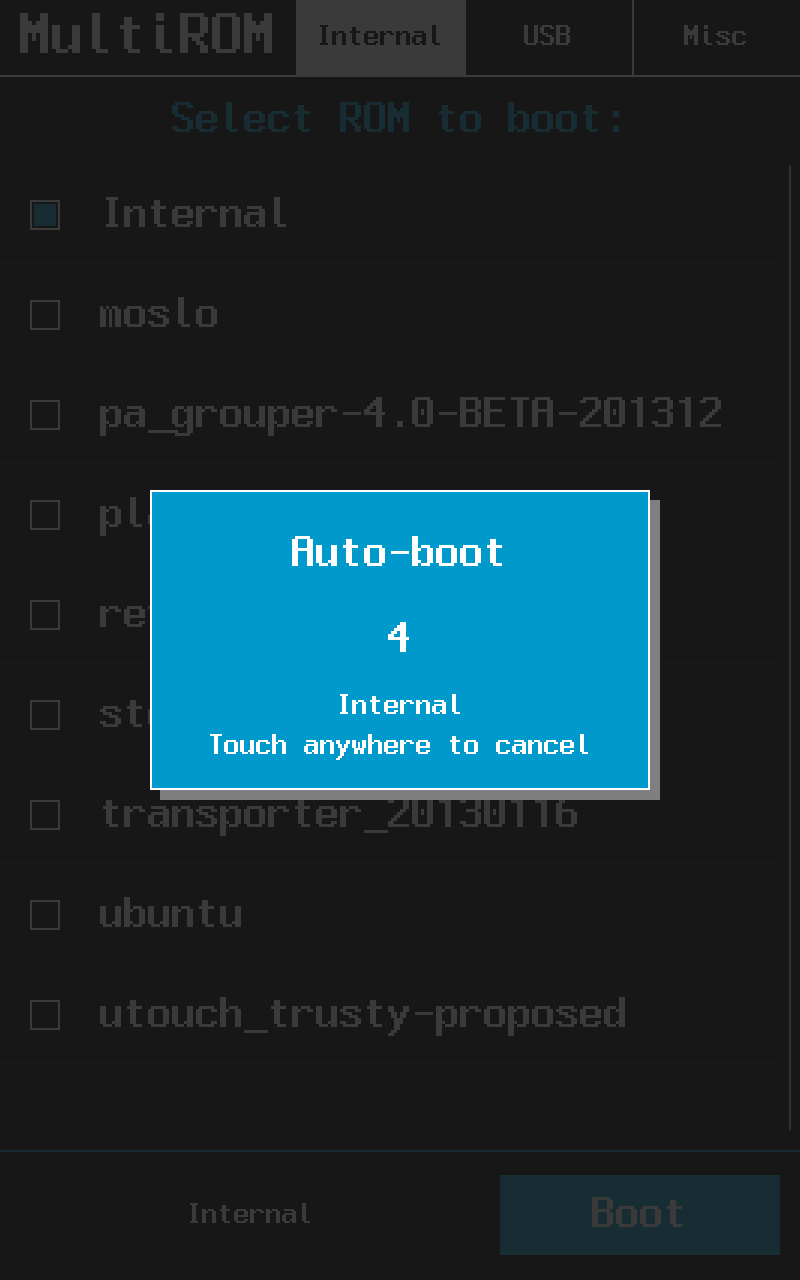
\includegraphics[height=550pt]{../img/boot_manager_autoboot.png}
\caption{Boot manager: je možné nastavit automatické spuštění jednoho ze systémů po určité prodlevě}
\end{center}
\end{figure}

\begin{figure}[H]
\begin{center}
 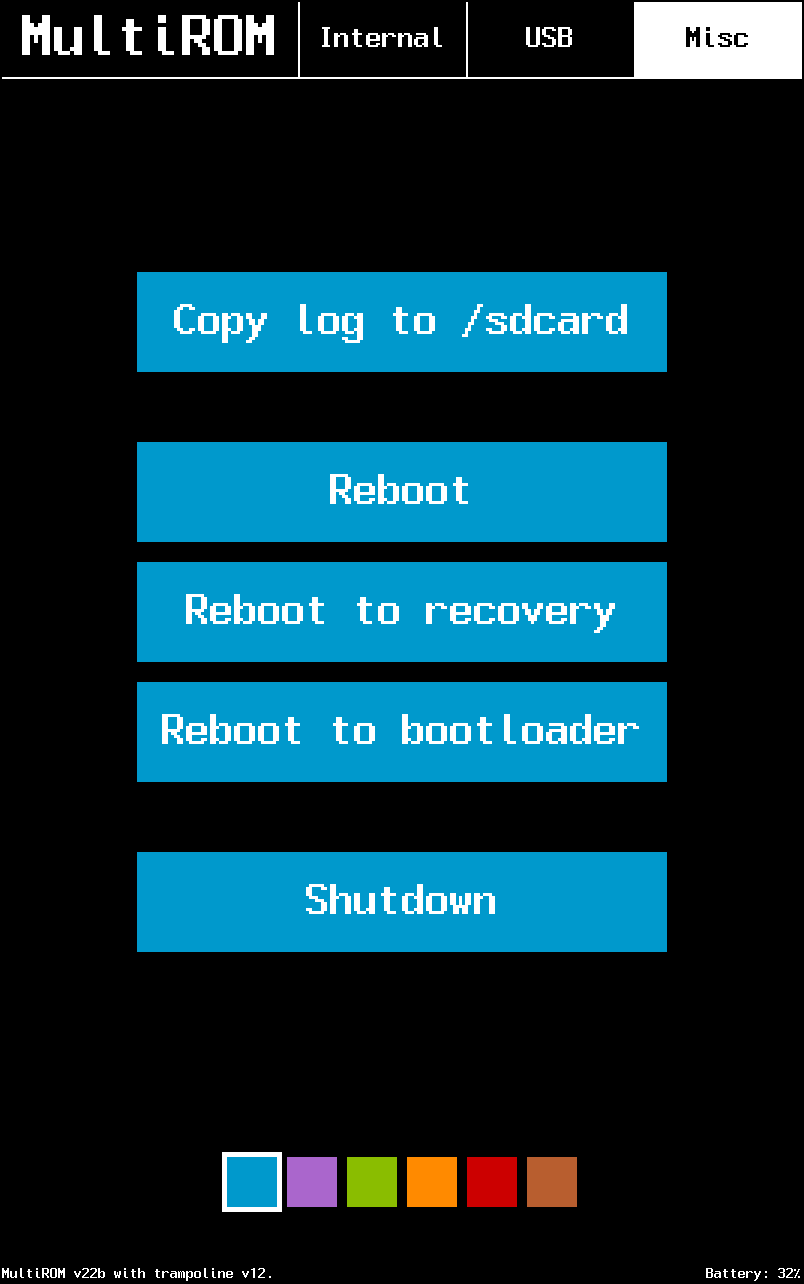
\includegraphics[height=550pt]{../img/boot_manager_misc.png}
\caption{Boot manager: obrazovka "ostatní možnosti"}
\end{center}
\end{figure}

\begin{figure}[H]
\begin{center}
 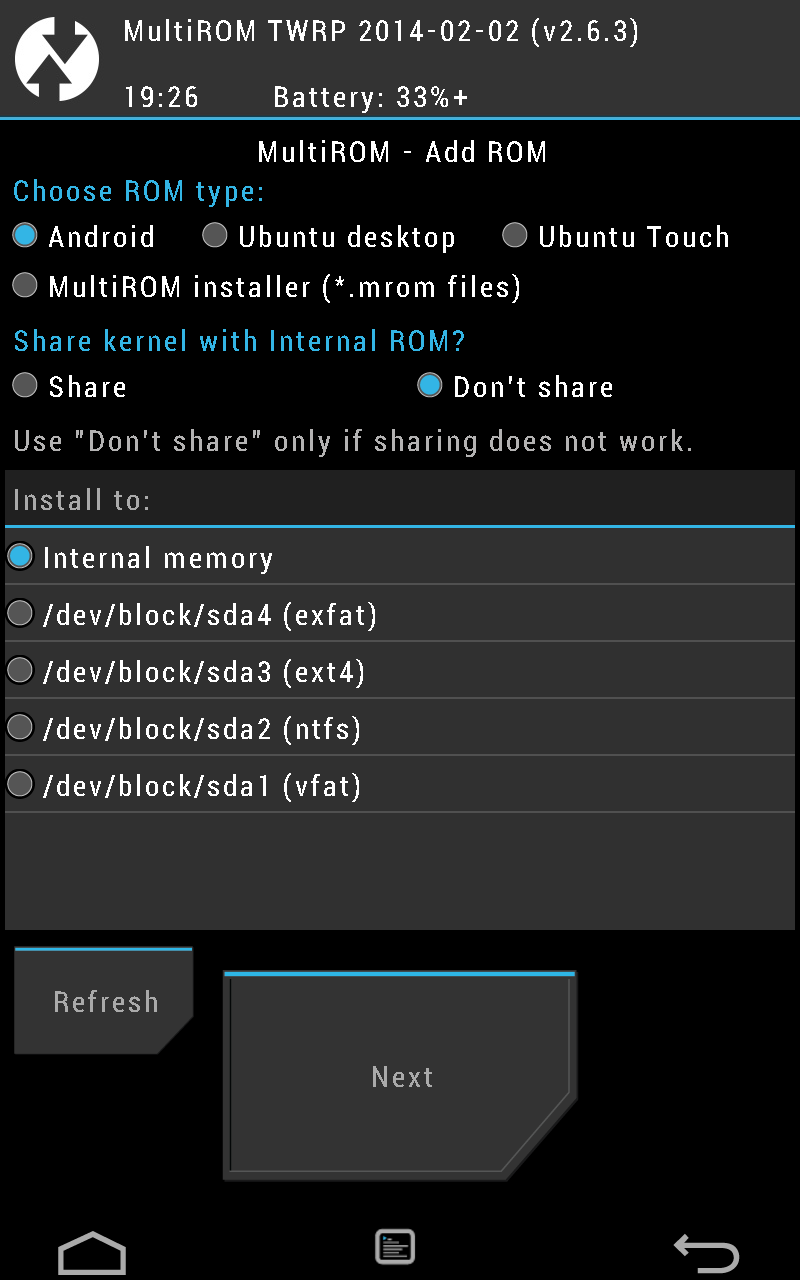
\includegraphics[height=550pt]{../img/recovery_install1.png}
\caption{Instalace vedlejšího systému v~recovery 1: výběr typu systému a~umístění instalace}
\end{center}
\end{figure}

\begin{figure}[H]
\begin{center}
 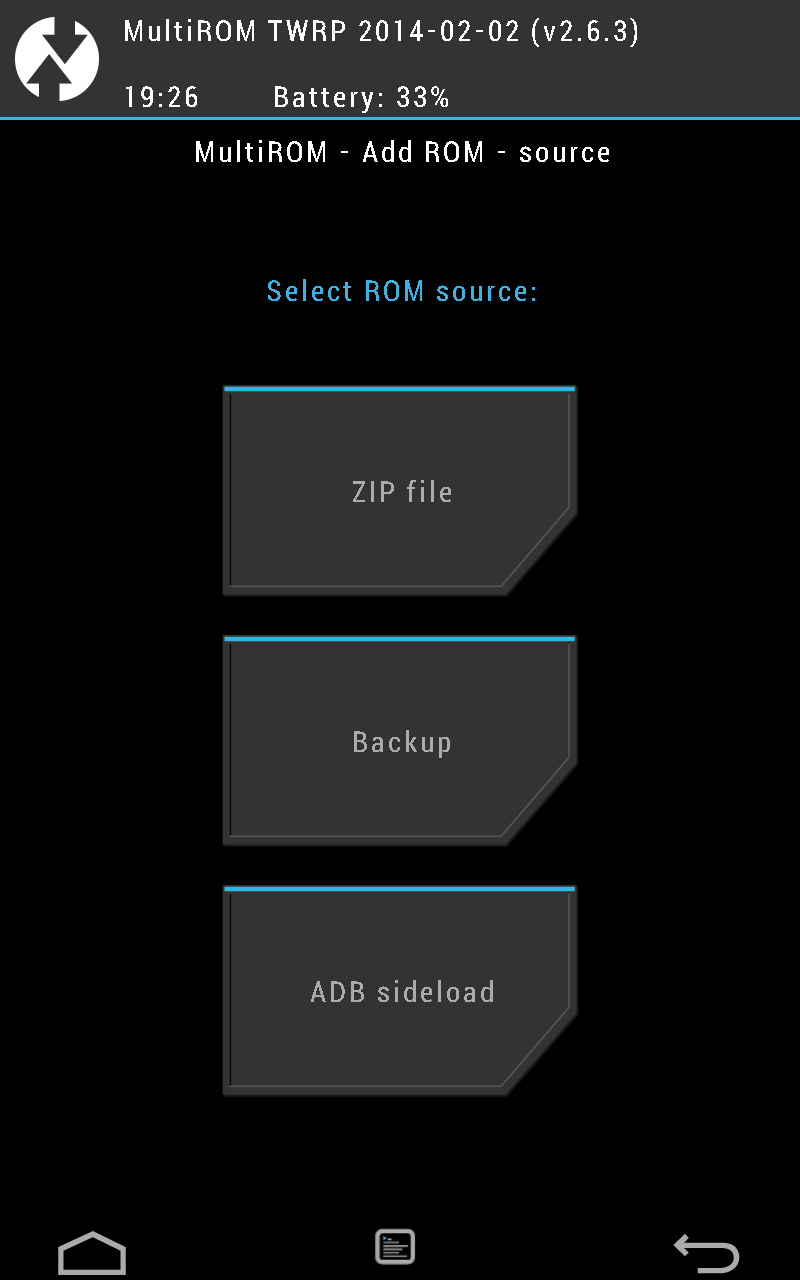
\includegraphics[height=550pt]{../img/recovery_install2.png}
\caption{Instalace vedlejšího systému v~recovery 2: výběr instalačního média (ZIP soubor, záloha nebo nahrání z~počítače přes USB)}
\end{center}
\end{figure}

\begin{figure}[H]
\begin{center}
 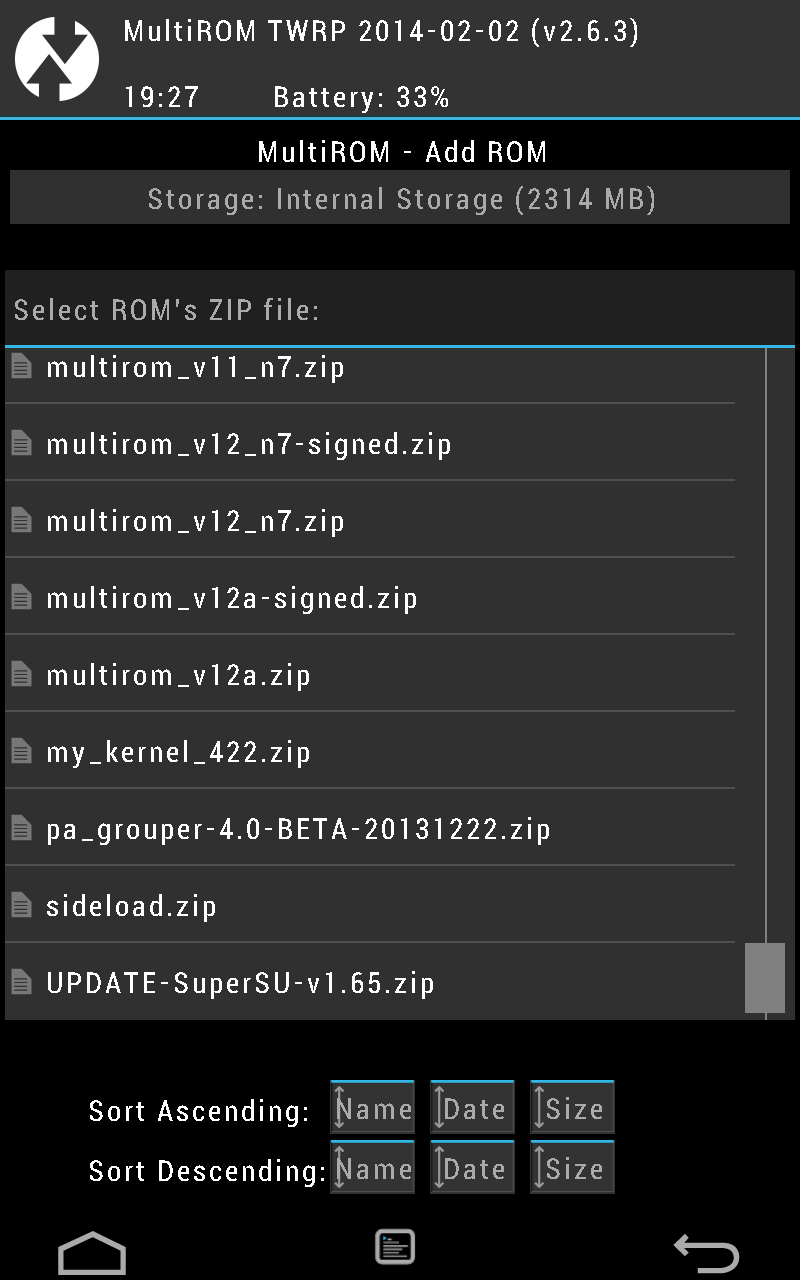
\includegraphics[height=550pt]{../img/recovery_install3.png}
\caption{Instalace vedlejšího systému v~recovery 3: výběr instalačního ZIP souboru}
\end{center}
\end{figure}

\begin{figure}[H]
\begin{center}
 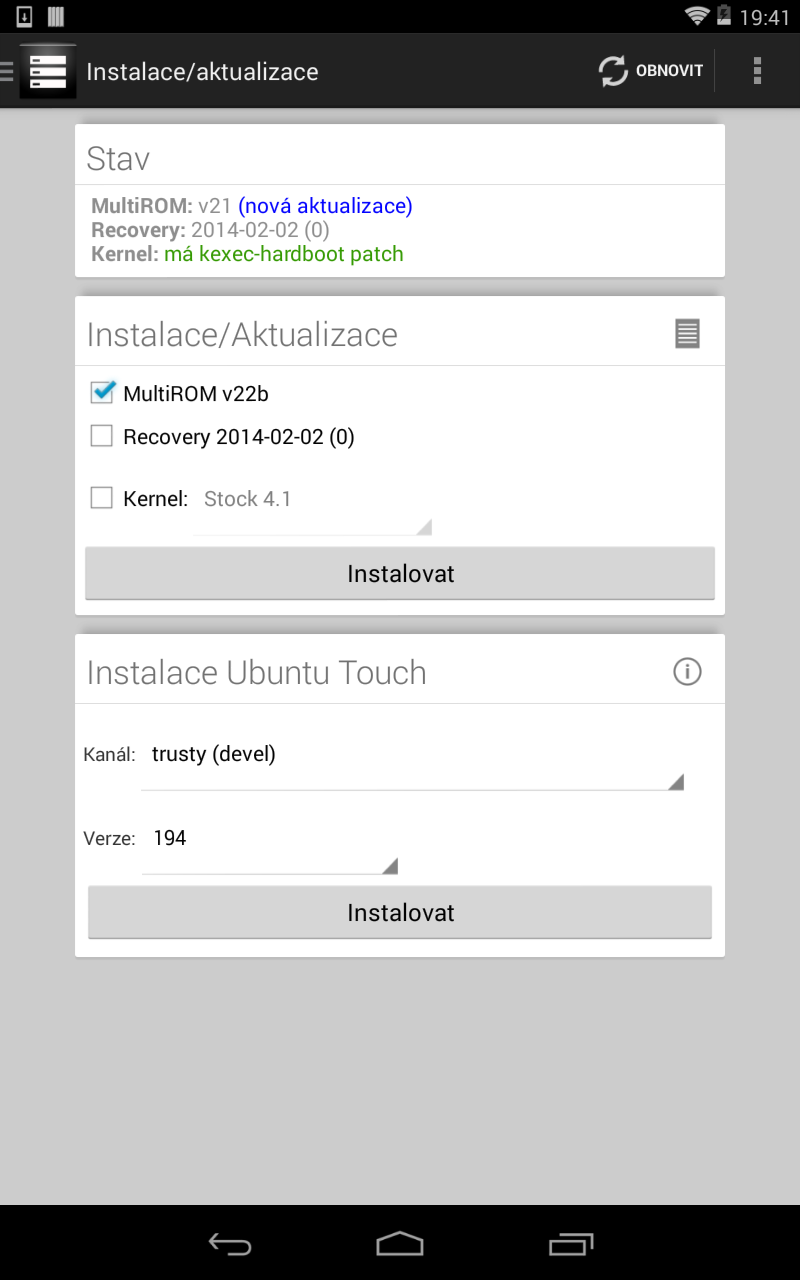
\includegraphics[height=550pt]{../img/app_main.png}
\caption{Android aplikace: hlavní obrazovka}
\end{center}
\end{figure}

\begin{figure}[H]
\begin{center}
 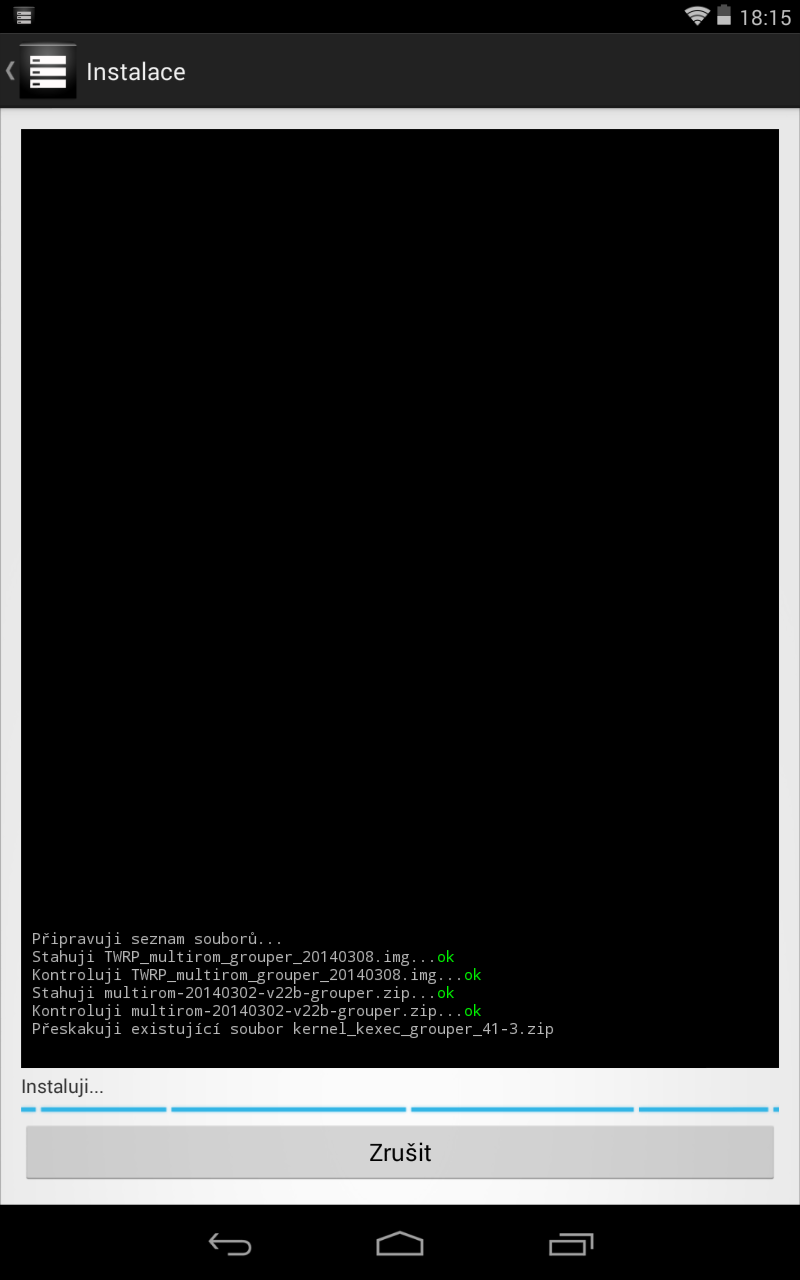
\includegraphics[height=550pt]{../img/app_install.png}
\caption{Android aplikace: probíhající instalace MultiROM}
\end{center}
\end{figure}

\begin{figure}[H]
\begin{center}
 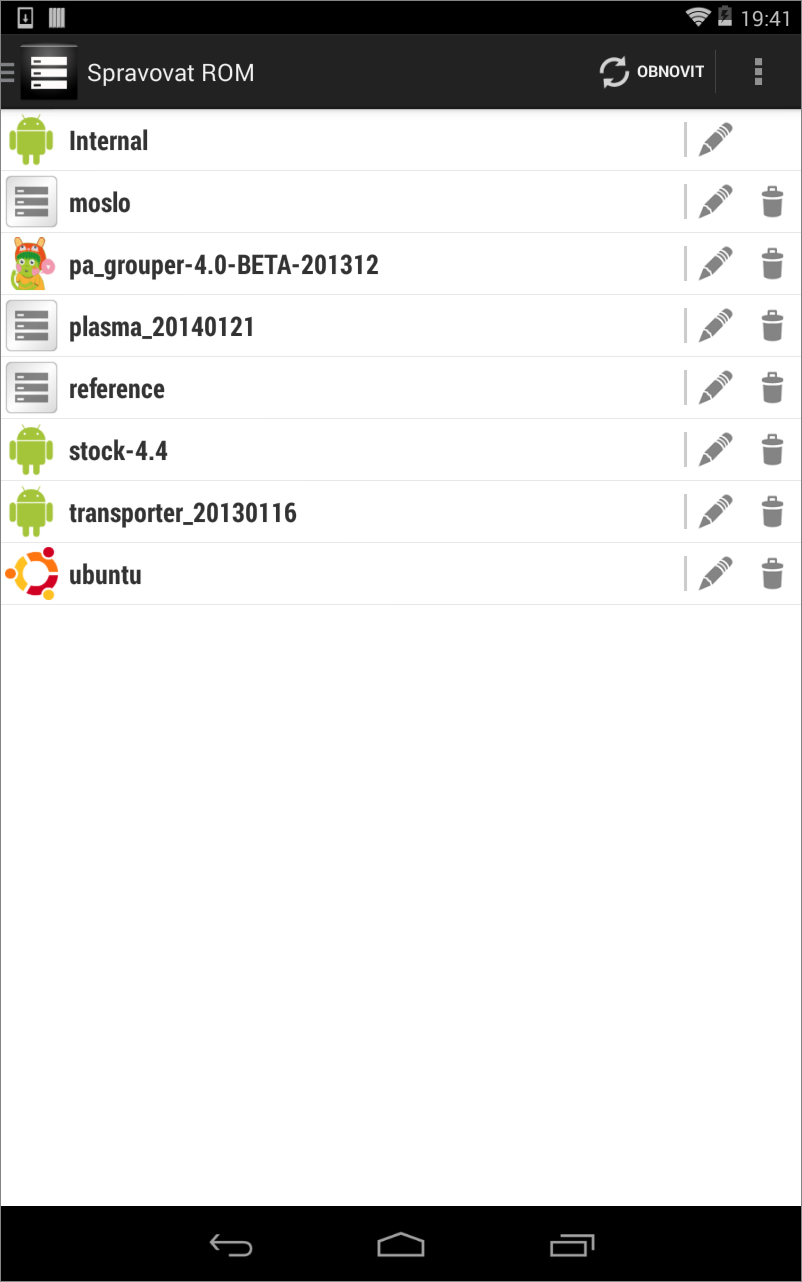
\includegraphics[height=550pt]{../img/app_roms.png}
\caption{Android aplikace: správa nainstalovaných systémů}
\end{center}
\end{figure}

\begin{figure}[H]
\begin{center}
 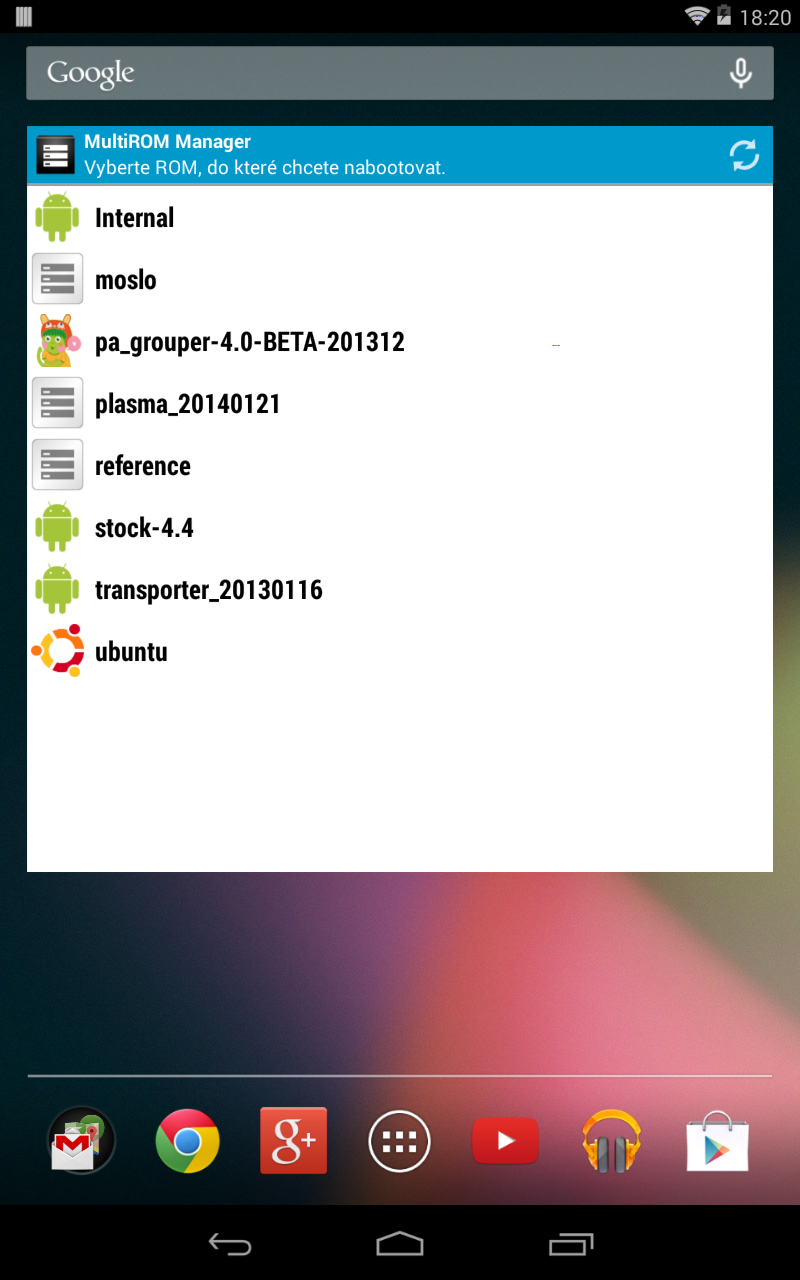
\includegraphics[height=550pt]{../img/app_widget.png}
\caption{Android aplikace: widget na plochu}
\end{center}
\end{figure}

\newpage
\section*{PŘÍLOHA B:}
\addcontentsline{toc}{section}{PŘÍLOHA B: Reference}
\printbibliography

\end{document}
